% =====================================================================
% GCC Corporate ESG Disclosure Quality: An Open Dataset and
% Transparent Scoring Methodology
% Author: Arafat Lakhani
% arXiv-ready: compiles with pdflatex + bibtex (or upload to Overleaf)
% All key statistics are macros defined in results/auto_results.tex,
% regenerated by analysis/analysis.py — never hard-code numbers here.
% =====================================================================
\documentclass[11pt]{article}
\usepackage[margin=1in]{geometry}
\usepackage{amsmath,amssymb}
\usepackage{booktabs}
\usepackage{graphicx}
\usepackage{hyperref}
\usepackage{natbib}
\usepackage{xcolor}
\usepackage{multirow}
\hypersetup{colorlinks=true, linkcolor=blue!60!black, citecolor=blue!60!black, urlcolor=blue!60!black}

% ---- Auto-generated statistics (run analysis/analysis.py to refresh) ----
% AUTO-GENERATED by analysis/analysis.py � do not edit by hand
\newcommand{\NComp}{21}
\newcommand{\NExch}{5}
\newcommand{\NCountry}{4}
\newcommand{\AvgDQS}{40.5}
\newcommand{\MedDQS}{37.5}
\newcommand{\SdDQS}{13.4}
\newcommand{\MaxDQS}{70.0}
\newcommand{\MinDQS}{15.0}
\newcommand{\ScopeThreePct}{10\%}
\newcommand{\AssurancePct}{81\%}
\newcommand{\NetZeroPct}{76\%}
\newcommand{\GriPct}{95\%}
\newcommand{\TcfdPct}{48\%}
\newcommand{\IssbPct}{43\%}
\newcommand{\MinSpearman}{0.923}


\newcommand{\todo}[1]{\textcolor{red}{[TODO: #1]}}
\newcommand{\dqs}{\textsc{dqs}}

\title{GCC Corporate ESG Disclosure Quality:\\
An Open Dataset and Transparent Scoring Methodology}

\author{Arafat Lakhani\\
\small Independent Researcher, Dubai, United Arab Emirates\\
\small \texttt{arafatilakhani@gmail.com}}

\date{July 2026 \\ \small Dataset and code: \url{https://github.com/ArafatL/gcc-esg-intelligence}}

\begin{document}
\maketitle

\begin{abstract}
Sustainability disclosure requirements are expanding rapidly across the
Gulf Cooperation Council (GCC), driven by ISSB-aligned regulatory roadmaps
and the United Arab Emirates' climate legislation. Yet no open,
company-level dataset exists against which the quality of GCC corporate
ESG disclosure can be measured, compared, or tracked: existing evidence is
locked inside commercial ratings whose methodologies are opaque and whose
outputs are known to diverge. We introduce an open dataset of ESG
disclosures from \NComp{} listed companies across \NExch{} GCC exchanges
(\NCountry{} countries), extracted from primary corporate reports using an
auditable, evidence-linked pipeline in which every value is traceable to
its source sentence and confirmed by human verification. We propose the
Disclosure Quality Score (\dqs{}), a deliberately transparent 0--100 index
of disclosure completeness and credibility whose every weight is public
and contestable. Applying \dqs{} to fiscal year 2024 reports, we find a
market average of \AvgDQS{}, with no company reaching the top
(``Leader'') band; Scope~3 emissions are disclosed by only \ScopeThreePct{}
of companies, and independent assurance remains the exception at
\AssurancePct{}. Disclosure quality varies systematically by sector and by
market. We release the dataset, extraction pipeline, and scoring code to
provide a reproducible baseline for tracking the GCC's disclosure
transition as ISSB adoption accelerates.
\end{abstract}

% =====================================================================
\section{Introduction}
% =====================================================================

The Gulf Cooperation Council economies are entering a structural
transition in corporate transparency. The IFRS Foundation's ISSB
standards (IFRS~S1 and~S2) have been finalised and jurisdictional
adoption roadmaps announced across the region
\citep{ifrs2023s1,ifrs2023s2}; the United Arab Emirates has enacted
federal climate legislation requiring greenhouse-gas measurement and
reporting by covered entities \citep{uaeclimatelaw2024}; and regional
exchanges---the Dubai Financial Market (DFM), Abu Dhabi Securities
Exchange (ADX), and the Saudi Exchange (Tadawul) among them---have issued
ESG disclosure guidance to their issuers. Capital is following the same
path: the region's sovereign wealth funds and banks have made
sustainable-finance commitments measured in the hundreds of billions of
dollars.

A transition of this scale requires measurement. Investors allocating to
GCC equities need to know which issuers disclose decision-useful
sustainability data; regulators need baselines against which to evaluate
the effect of new mandates; issuers need peer benchmarks; and researchers
need data. Yet the empirical foundation is missing. Commercial ESG
ratings cover only the largest GCC issuers, their methodologies are
proprietary, and a substantial literature documents that their outputs
disagree with one another to a degree that undermines their use as
measurement instruments \citep{berg2022aggregate}. Meanwhile, the raw
material---corporate sustainability reports---is public but unusable at
scale: hundreds of pages of PDF per company per year, with key metrics
embedded in heterogeneous tables.

This paper makes three contributions:

\begin{enumerate}
\item \textbf{An open dataset.} We construct and release a
company-level dataset of ESG disclosures for \NComp{} listed companies
across the DFM, ADX, Tadawul, Qatar Stock Exchange, and Boursa Kuwait,
covering nine core quantitative metrics (Scope~1/2/3 emissions, energy,
water, renewable share, female workforce share, board independence, and
workforce nationalisation) and eight credibility signals (framework
alignment, net-zero targets, external assurance) for fiscal year 2024.
To our knowledge this is the first openly licensed, company-level ESG
disclosure dataset for GCC markets.
\item \textbf{An auditable measurement methodology.} Every extracted
value in the dataset is linked to the sentence of the source report from
which it was taken and passes a documented human-verification protocol.
We argue this evidence-traceability property---absent from both
commercial ratings and most LLM-based extraction systems---is a
precondition for disclosure data that can support regulatory and academic
use.
\item \textbf{A transparent disclosure-quality index.} We define the
Disclosure Quality Score (\dqs{}), a 0--100 composite of disclosure
\emph{coverage}, \emph{framework alignment}, and \emph{credibility
rigor}. Unlike commercial ESG ratings, \dqs{} measures the quality of
\emph{disclosure}, not the sustainability of \emph{performance}, and its
weights are published, justified, and subjected to sensitivity analysis.
\end{enumerate}

Applying the methodology to FY2024 reports yields the first open
market-wide picture of GCC disclosure quality. The average \dqs{} is
\AvgDQS{} of 100. No company reaches the Leader band ($\geq 75$),
indicating that even the region's most celebrated sustainability
reporters leave material gaps---most commonly Scope~3 emissions
(disclosed by \ScopeThreePct{} of companies) and independent assurance
(obtained by \AssurancePct{}). Banks and telecommunications firms
disclose most completely; \todo{confirm sector finding on final verified
data}. We discuss implications for regulators designing ISSB adoption
sequences and for investors interpreting the region's sustainability
claims.

% =====================================================================
\section{Related Work}
% =====================================================================

\paragraph{Disclosure indices in accounting research.}
Measuring disclosure through structured content analysis has a long
tradition in accounting scholarship. Self-constructed disclosure indices
---checklists of items scored for presence and quality---underpin classic
studies of voluntary disclosure and its capital-market consequences
\citep{marston1991use,botosan1997disclosure}, and mandatory-reporting
reviews emphasise that index transparency is what makes findings
interpretable and replicable \citep{christensen2021mandatory}. \dqs{}
stands in this tradition: it is a modern, machine-assisted disclosure
index whose item list, weights, and evidence are public. What is new is
the scale and auditability that automated extraction makes possible.

\paragraph{ESG rating divergence.}
\citet{berg2022aggregate} document that commercial ESG ratings of the
same firm correlate only moderately across providers, driven by
differences in scope, measurement, and weights---none of which are
observable to users. This ``aggregate confusion'' motivates our design
choice to measure a narrower construct (disclosure quality) with fully
observable methodology, rather than a broader construct (ESG performance)
with hidden machinery.

\paragraph{LLM-based ESG information extraction.}
A fast-growing NLP literature extracts structured ESG data from
sustainability reports. ESGReveal combines large language models with
retrieval-augmented generation to extract metrics from ESG reports
\citep{esgreveal}; ESG-KG constructs knowledge graphs from sustainability
reports with evidence chains for compliance evaluation \citep{esgkg};
and ESGAgent orchestrates hierarchical LLM agents over hundreds of
corporate reports \citep{esgagent}. These systems demonstrate technical
feasibility but share two limitations from a measurement perspective:
their outputs are not released as open, verified datasets, and their
coverage concentrates on US, European, and East Asian issuers. Notably,
this literature itself observes the absence of publicly available ESG
disclosure databases with detailed metric coverage \citep{esgreveal}. We
complement it from the data side: a deliberately simple, auditable
extraction pipeline (pattern-based, table-aware, with optional LLM
assistance) whose output is a verified public dataset for a region the
literature has not covered.

\paragraph{Assurance and credibility.}
External assurance of sustainability reports is associated with
credibility and is unevenly adopted across jurisdictions
\citep{simnett2009assurance}. Our rigor pillar operationalises
credibility signals---assurance, quantified net-zero commitment, and
value-chain (Scope~3) transparency---as scored components.

% =====================================================================
\section{Data}
% =====================================================================

\subsection{Company registry}
The registry covers \NComp{} listed companies: \todo{final split}
United Arab Emirates (DFM and ADX), Saudi Arabia (Tadawul), Qatar (QSE),
and Kuwait (Boursa Kuwait), selected to span the region's dominant
sectors---banking, telecommunications, energy, utilities, real estate,
chemicals, industrials, mining, and transport infrastructure. Selection
prioritised index heavyweights and sustainability-report availability;
we discuss the resulting selection bias in Section~\ref{sec:limitations}
(the sample over-represents large, visible issuers, so market-wide
averages should be read as an \emph{upper bound} on typical disclosure
quality).

\subsection{Source documents}
For each company we identified the FY2024 sustainability report, ESG
data pack, or integrated annual report from the issuer's investor
relations site or exchange disclosure feed. Every source URL was
verified to resolve to a live PDF and is recorded in the dataset
(\texttt{companies.csv}), making the entire corpus re-downloadable.
Document sourcing quirks (exchange feeds, mirror repositories,
non-standard paths) are documented in the project's extraction log to
support replication.

\subsection{Extraction pipeline}
\label{sec:pipeline}
Documents are converted to text and passed through a pattern-based
extraction engine targeting nine quantitative metrics and eight
credibility signals. Two design lessons from GCC documents shaped the
engine. First, metrics appear predominantly in \emph{table} layouts in
which the unit lives in a column header rather than beside the value
(e.g., ``Emission Category in tCO\textsubscript{2}e \ldots\ Scope~1 \quad
757.78''); patterns therefore exist in sentence-style and table-style
variants. Second, units are heterogeneous (kWh vs.\ MWh, litres vs.\
m\textsuperscript{3}); every pattern carries an explicit unit conversion.
Each extracted value retains an \emph{evidence snippet}---the surrounding
source text---so that any number in the dataset can be traced to the
sentence that produced it. An optional LLM-assisted extractor handles
documents that defeat pattern matching; its outputs pass the same
evidence and verification requirements.

\subsection{Human verification protocol}
\label{sec:verification}
Automated extraction is a recall device, not a ground truth. Every row
in the released dataset carries a verification status; a row is marked
\texttt{verified} only after a human validator has compared each
extracted value against the source PDF and logged the page number. As a
worked example, the Emirates NBD Group FY2024 data pack yields Scope~1
emissions of 757.78~tCO\textsubscript{2}e, Scope~2 of 36{,}271.17, and
Scope~3 (eight categories) of 199{,}795.04, each carrying limited
assurance by a Big Four auditor under ISAE~3000/3410---values our
pipeline extracts and links to their source table, and which human
verification confirms. \todo{report inter-verification agreement
statistics once second-pass checks are complete}

% =====================================================================
\section{The Disclosure Quality Score}
% =====================================================================
\label{sec:dqs}

\subsection{Definition}
For company $i$, let $M_i \subseteq \mathcal{M}$ be the set of core
quantitative metrics disclosed (of $|\mathcal{M}| = 9$), $F_i \subseteq
\mathcal{F}$ the set of reporting frameworks referenced (of
$|\mathcal{F}| = 6$: GRI, TCFD, ISSB/IFRS~S1--S2, SASB, CDP, UN SDGs),
and let $a_i$, $z_i$, $s_i$ be indicators for external assurance, a
stated net-zero target, and Scope~3 disclosure respectively. Then
\begin{equation}
\dqs{}_i \;=\;
\underbrace{45 \cdot \frac{|M_i|}{9}}_{\text{Coverage}}
\;+\;
\underbrace{30 \cdot \frac{|F_i|}{6}}_{\text{Frameworks}}
\;+\;
\underbrace{\min\bigl(10\,a_i + 7.5\,z_i + 7.5\,s_i,\; 25\bigr)}_{\text{Rigor}} .
\label{eq:dqs}
\end{equation}
Scores map to four bands: Leader ($\geq 75$), Advanced ($\geq 50$),
Developing ($\geq 25$), Minimal ($< 25$).

\subsection{What \dqs{} is and is not}
\dqs{} measures whether an investor can \emph{find} decision-useful
sustainability data in a company's reporting---not whether the company's
sustainability performance is good. A high-emitting firm that discloses
completely, under assurance, scores higher than a low-emitting firm that
discloses nothing. This is intentional: conflating disclosure with
performance is precisely the ambiguity that makes commercial ratings
divergent and hard to interpret \citep{berg2022aggregate}. Disclosure
quality is also the construct regulators directly govern.

\subsection{Weight justification and sensitivity}
Coverage receives the largest weight (45) because quantitative metric
availability is the primary user need and the binding constraint for any
downstream analysis. Frameworks (30) proxy reporting maturity and
comparability: alignment with GRI, TCFD, or ISSB commits an issuer to
defined disclosure architectures. Rigor (25) rewards credibility
mechanisms, with assurance weighted highest within the pillar given
evidence on its credibility role \citep{simnett2009assurance}; Scope~3
appears in Rigor rather than Coverage because value-chain accounting
demands a step-change in capability and is the sharpest discriminator
among otherwise-complete disclosers.

Any fixed weighting is contestable, so we treat robustness as an
empirical question: Section~\ref{sec:sensitivity} re-scores the market
under systematic weight perturbations and reports rank stability. The
scoring code is public; users who disagree with our weights can re-score
the dataset under their own in one line.

% =====================================================================
\section{Results}
% =====================================================================
\label{sec:results}

\noindent\emph{All statistics in this section are generated by
\texttt{analysis/analysis.py} from the verified dataset and injected as
macros; the numbers below refresh automatically when the verified panel
is finalised.}

\subsection{Market-level disclosure quality}
Across \NComp{} companies, mean \dqs{} is \AvgDQS{} (median
\MedDQS{}, s.d.\ \SdDQS{}). No company attains the Leader band; the
highest score is \MaxDQS{} and the lowest \MinDQS{}. The market
distribution concentrates in the Developing and Advanced bands
(Figure~\ref{fig:ranking}), implying that GCC sustainability reporting
has broadly moved past minimal, boilerplate disclosure but has not yet
reached the completeness-plus-credibility frontier that ISSB-aligned
regimes will demand.

\begin{figure}[t]
\centering
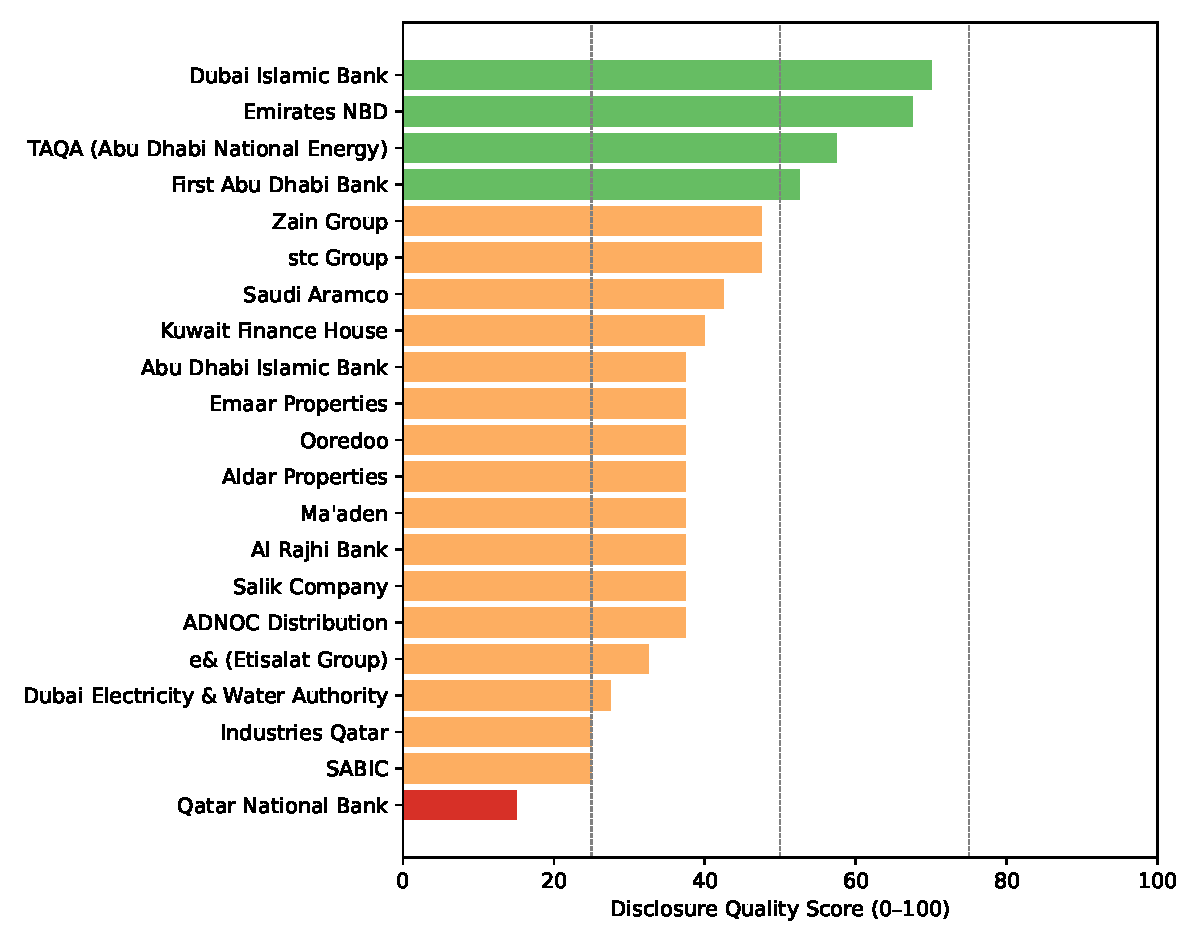
\includegraphics[width=\textwidth]{figures/fig1_ranking.pdf}
\caption{Disclosure Quality Scores by company, FY2024, coloured by band.}
\label{fig:ranking}
\end{figure}

\subsection{Where disclosure fails: the coverage anatomy}
Figure~\ref{fig:coverage} decomposes coverage by metric. Scope~1 and
Scope~2 emissions and headline social metrics are now widely disclosed;
the gaps are concentrated in Scope~3 emissions (\ScopeThreePct{} of
companies), \todo{water/renewables findings}, and quantified
board-independence figures. External assurance is obtained by
\AssurancePct{} of companies, and \NetZeroPct{} state a net-zero target.
The pattern is consistent with a market in the ``framework adoption''
phase of the disclosure transition: reference to GRI is near-universal
(\GriPct{}), TCFD alignment substantial (\TcfdPct{}), and ISSB reference
emerging (\IssbPct{}) ahead of mandatory timelines.

\begin{figure}[t]
\centering
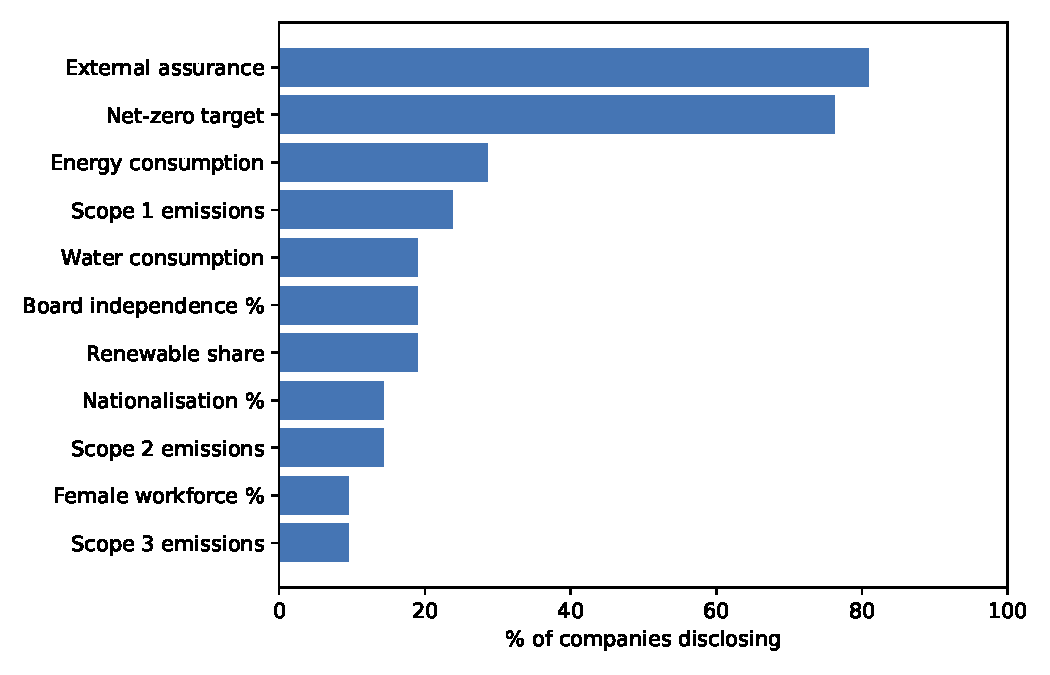
\includegraphics[width=.9\textwidth]{figures/fig2_coverage.pdf}
\caption{Share of companies disclosing each core metric and credibility signal.}
\label{fig:coverage}
\end{figure}

\subsection{Sector and market patterns}
\begin{table}[t]\centering
\caption{Disclosure quality by sector.}\label{tab:sector}
\begin{tabular}{lrrrr}\toprule
Sector & $n$ & Mean \dqs{} & Scope~3 & Assured \\ \midrule
Banking & 7 & 45.7 & 29\% & 71\% \\
Utilities & 2 & 42.5 & 0\% & 100\% \\
Telecom & 4 & 41.2 & 0\% & 50\% \\
Energy & 2 & 40.0 & 0\% & 100\% \\
Mining & 1 & 37.5 & 0\% & 100\% \\
Real Estate & 2 & 37.5 & 0\% & 100\% \\
Transport Infrastructure & 1 & 37.5 & 0\% & 100\% \\
Industrials & 1 & 25.0 & 0\% & 100\% \\
Chemicals & 1 & 25.0 & 0\% & 100\% \\
\bottomrule\end{tabular}\end{table}

\begin{table}[t]\centering
\caption{Disclosure quality by market.}\label{tab:country}
\begin{tabular}{lrrrr}\toprule
Country & $n$ & Mean \dqs{} & Scope~3 & Assured \\ \midrule
UAE & 11 & 45.0 & 18\% & 82\% \\
KUWAIT & 2 & 43.8 & 0\% & 100\% \\
KSA & 5 & 38.0 & 0\% & 80\% \\
QATAR & 3 & 25.8 & 0\% & 67\% \\
\bottomrule\end{tabular}\end{table}

Banks and telecommunications issuers---sectors with the longest exposure
to international investors and regulatory reporting---disclose most
completely. \todo{Interpret sector/country table once verified panel is
final; candidate narrative: financial-sector supervisory pressure and
regional flagship effects.}

\subsection{Weight sensitivity}
\label{sec:sensitivity}
We re-score all companies under perturbed weightings in which 10 points
are transferred between each pair of pillars, and under equal weighting.
Spearman rank correlation between baseline and perturbed rankings is
\MinSpearman{} at minimum across perturbations
(Figure~\ref{fig:sensitivity}), indicating that the ordering---though not
the absolute scores---is robust to reasonable disagreement about weights.

\begin{figure}[t]
\centering
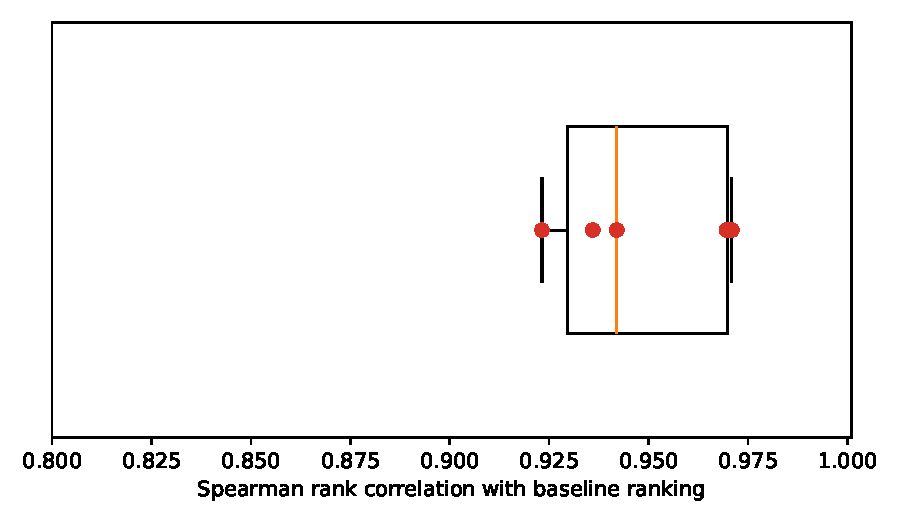
\includegraphics[width=.75\textwidth]{figures/fig3_sensitivity.pdf}
\caption{Rank stability of \dqs{} under weight perturbations.}
\label{fig:sensitivity}
\end{figure}

% =====================================================================
\section{Discussion}
% =====================================================================

\paragraph{For regulators.} The coverage anatomy offers a sequencing
map: mandating Scope~1/2 disclosure would formalise near-existing
practice, whereas Scope~3 and assurance mandates would bind. Baselines
such as \dqs{} allow the effect of the UAE climate law and ISSB adoption
to be measured rather than asserted; the dataset's FY2024 vintage
constitutes a pre-mandate baseline.

\paragraph{For investors.} The absence of any Leader-band issuer
cautions against equating regional sustainability marketing with
disclosure completeness. Because every \dqs{} point is traceable to
evidence, the score can be used in engagement: an investor can ask a
specific issuer for the specific missing items.

\paragraph{For the measurement literature.} Our results illustrate that
useful disclosure measurement does not require opaque
machinery. A transparent index over verified extractions supports
stronger claims---about disclosure---than black-box ratings support about
performance.

% =====================================================================
\section{Limitations and Future Work}
% =====================================================================
\label{sec:limitations}
Our sample is small (\NComp{} companies) and selects on size and report
availability; results bound typical disclosure quality from above and
are not market-representative in the statistical sense. The current
release covers a single fiscal year; the pipeline and located historical
reports (2020--2024) support extension to a panel, which is our immediate
next step and will permit trend and event-style analyses around
regulatory milestones. Extraction is English-only, excluding
Arabic-only reporters---a coverage bias we intend to remove with
Arabic-language support. Pattern-based extraction favours precision over
recall: a metric disclosed in an unusual format may be missed, which
human verification mitigates but cannot eliminate. Finally, \dqs{}
weights, though published and sensitivity-tested, remain judgments; we
release scoring code precisely so alternatives can be computed.

% =====================================================================
\section{Conclusion}
% =====================================================================
We release the first open, evidence-linked, human-verified dataset of
corporate ESG disclosure for GCC markets, together with a transparent
scoring methodology and its full pipeline. The FY2024 baseline shows a
region mid-transition: broad framework adoption and headline-metric
disclosure, but material gaps in value-chain emissions and assurance,
and no issuer yet at the completeness frontier. As ISSB-aligned mandates
arrive, this baseline---and the open infrastructure behind it---enables
the GCC's disclosure transition to be tracked in public.

\paragraph{Data and code availability.}
Dataset, extraction pipeline, scoring code, and analysis scripts are
available under the MIT licence at
\url{https://github.com/ArafatL/gcc-esg-intelligence}; the versioned
dataset release carries a DOI via Zenodo. \todo{insert DOI after
Zenodo deposit}

\paragraph{Ethics and competing interests.}
All data derive from public corporate disclosures; no personal data are
processed. The author declares no competing interests. \todo{add
acknowledgements if any}

\bibliographystyle{plainnat}
\bibliography{refs}

\appendix
\section{Metric and Signal Definitions}
\begin{tabular}{ll}\toprule Item & Dataset column \\ \midrule
Scope 1 emissions & \texttt{scope1\_emissions\_tco2e} \\
Scope 2 emissions & \texttt{scope2\_emissions\_tco2e} \\
Scope 3 emissions & \texttt{scope3\_emissions\_tco2e} \\
Energy consumption & \texttt{energy\_consumption\_mwh} \\
Water consumption & \texttt{water\_consumption\_m3} \\
Renewable share & \texttt{renewable\_energy\_pct} \\
Female workforce \% & \texttt{female\_workforce\_pct} \\
Board independence \% & \texttt{board\_independence\_pct} \\
Nationalisation \% & \texttt{emiratisation\_pct} \\
External assurance & \texttt{fw\_assurance} \\
Net-zero target & \texttt{fw\_net\_zero\_target} \\
\bottomrule\end{tabular}


\section{Verification Protocol}
Each extracted value is compared against the source PDF by a human
validator; the validator records the page number, confirms unit and
entity scope (group vs.\ parent), and marks the row \texttt{verified} or
corrects it with a note. Corrections feed pattern improvements, which
are logged with dates in the public extraction log.

\end{document}
